\documentclass[10pt,a4paper]{article}
\usepackage[utf8]{inputenc} % para poder usar tildes en archivos UTF-8
\usepackage[spanish]{babel} % para que comandos como \today den el resultado en castellano
\usepackage{a4wide} % márgenes un poco más anchos que lo usual
\usepackage[conEntregas]{caratula}
\usepackage{amssymb}
\usepackage{amsthm}
\usepackage{fancybox}
\usepackage[usenames,dvipsnames]{color}
\usepackage{hyperref}
\usepackage{listings}
\usepackage{ulem}
\usepackage{color}
\usepackage[table]{xcolor}
\usepackage{amsmath}
\usepackage{float}
\usepackage{pdflscape}
%\usepackage[landscape]{geometry}
\usepackage{pdfpages}
\usepackage{algorithmic}


\hypersetup{
    colorlinks,
    citecolor=black,
    filecolor=black
    linkcolor=black,
    urlcolor=black
}

\lstdefinestyle{customc}{
  belowcaptionskip=1\baselineskip,
  breaklines=true,
  frame=L,
  xleftmargin=\parindent,
  language=C,
  showstringspaces=false,
  basicstyle=\footnotesize\ttfamily,
  keywordstyle=\bfseries\color{green!40!black},
  commentstyle=\itshape\color{purple!40!black},
  identifierstyle=\color{blue},
  stringstyle=\color{orange},
}

\newtheorem{theorem}{Teorema}[section]
\newtheorem{corollary}{Corolario}[theorem]
\newtheorem{lemma}[theorem]{Lema}
\newtheorem{definition}[theorem]{Definicion}

\newcommand{\norm}[1]{\left\lVert#1\right\rVert}

\newcommand{\BigO}[1]{\ensuremath{\operatorname{O}\bigl(#1\bigr)}}
\newtheorem{proposition}{Proposici\'on}

\begin{document}

\titulo{Primer parcial}

\fecha{\today}

\materia{Algoritmos y Estructuras de Datos Avanzadas}

\integrante{Vileriño, Silvio}{106/12}{svilerino@gmail.com}

\maketitle

\tableofcontents
\newpage

\section{Ejercicio 1}

\subsection{Item a)}
\textbf{Idea de la demostracion:} Supongamos que sabemos convertir una instancia de set-cover en una instancia de clique transversal sobre grafo split, que una solucion a CT sobre dicho grafo contiene solamente nodos de la parte clique del grafo split y que se puede convertir a una solucion de la instancia set-cover asociada al grafo.\\

De esta forma, si existiera un algoritmo $\alpha-aproximado$ podríamos resolver set-cover con el, lo cual es absurdo ya que set-cover no es $\alpha-aproximable$\footnote{Lo vimos en clase.}.\\

Veamos que contiene una instancia $I_{sc}$ de set cover:
\begin{itemize}
    \item Sea un universo de elementos $U = \{e_1, \dots, e_m\}$
    \item Sea $S = \{S_1, \dots, S_n\}$ un conjunto tal que $S_i \subseteq U$ y además $\bigcup\limits_{s_i \in S} s_{i} = U$
\end{itemize}

Nuestro objetivo es convertir $ I_{sc} $ en un grafo split \footnote{$https://en.wikipedia.org/wiki/Split_graph$}.\\

Consideremos el siguiente grafo basado en una instancia $I_{sc}$ de Set Cover:
\begin{itemize}
    \item Sea G = (V, E) un grafo split, donde V = $V_{indep}$ $\dot{\cup}$ $V_{clique}$.
    \item Sean los nodos de $V_{indep}$ una biyección con los elementos del universo U de Set Cover.
    \item Sean los nodos de $V_{clique}$ una biyección con los elementos del conjunto S de Set Cover.
    \item Las aristas del grafo G son:
    \begin{itemize}
        \item Sean $v \in V_{indep}$, $w \in V_{clique}$, existe la arista $(v, w) \in E$ si y solo si $v \in w$ en el contexto de elementos de Set Cover\footnote{Es decir, el elemento $v \in U$ está en el conjunto $w \in S$ o análogamente $w \in S$ contiene al elemento $v \in U$}.
        \item Se clausuran las aristas de la parte clique del grafo split para que, justamente sea una clique respetando la definición de grafo split.
    \end{itemize}
    \item En nuestro caso, ya que los elementos del universo U estan cubiertos por la union de los elementos de S, no habra nodos aislados en $V_{indep}$ 
\end{itemize}

\begin{figure}[H]
    \centering
    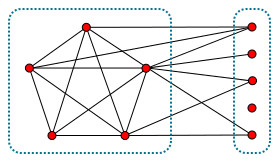
\includegraphics[scale=0.75]{fig/Split_graph.jpg}
    \label{fig:split_graph}
    \caption{Ejemplo de grafo split.}
\end{figure}

\begin{proposition}
Sea $CT_{opt}$ un clique transversal minimo sobre un grafo split $G = (V, E)$, de cardinal $L$, se puede construir una nueva solucion $CT'_{opt}$ de mismo cardinal, pero solo conteniendo nodos de $V_{clique}$. De ahora en mas, asumimos soluciones de estas caracteristicas para el resto de la demostracion.
\end{proposition}

\begin{proof}
Sea $I = V_{indep} \cap CT_{opt}$, puede verse que ningun par de nodos $v, w \in I$ tienen un vecino en comun, caso contrario podrian removerse v,w y agregarse dicho vecino en comun a la solucion, produciendo un clique transversal de menor cardinal, lo que es absurdo, pues dijimos que tenia cardinal minimo. \\
Por otra parte, ningun nodo $v \in I$ tiene por vecino a un nodo $w \in CT{opt}$, de lo contrario, podria removerse v de $CT_{opt}$ y lograr nuevamente una solucion de cardinal menor al minimo, cometiendo un absurdo. Dadas estas ultimas dos afirmaciones, proponemos el siguiente metodo para generar una solucion $CT'_{opt}$ de mismo cardinal conteniendo solo nodos de $V_{clique}$:\\


\begin{algorithmic}
    \STATE $CT'_{opt} \gets CT_{opt}$
    \STATE $I \gets V_{indep} \cap CT_{opt}$
    \FOR{$v \in I$}
        \STATE $CT'_{opt} \gets \setminus \{v\}$
        \STATE $CT'_{opt} \gets CT'_{opt} \cup {vecino(v)}$
    \ENDFOR
\end{algorithmic}

Veamos que ademas, la funcion vecino(v), que devuelve cualquier vecino de $v \in I$ no se indefine, pues $v$ no puede ser un nodo aislado al pertenecer a la solucion $CT_{opt}$. \\
Finalmente, consideremos $w = vecino(v)$. Como G es un grafo split, y $v \in I \subseteq V_{indep}$, necesariamente debe ser $w \in V_{clique}$.\\
Al finalizar el algoritmo, $CT'_{opt}$ tiene mismo cardinal que $CT_{opt}$ y ademas solo contiene nodos $t \in V_{clique}$ como queriamos.
\end{proof}

\begin{proposition}
 Considerando en el contexto de set cover: Los conjuntos denotados por los nodos de la solucion de $CT_{opt} \subseteq V_{clique}$, constituyen una solucion minima para Set Cover.
\end{proposition}

\begin{proof}
Sea $CT_{opt}$ una solución minima para clique transversal sobre este grafo G que armamos en base a $I_{SC}$. Sea $SC_{opt}$ una solucion minima de Set Cover para la instancia $I_{SC}$ de \textbf{de cardinal menor} a $CT_{opt}$.\\

Consideremos $V_{SC} $ los nodos del grafo split asociados a los elementos de $SC_{opt}$. Como la solucion de set cover cubre todo el universo, en contexto del grafo G, todos los nodos de $V_{indep}$ seran adyacentes con alguno de $V_{SC}$.\\
Por otro lado, al considerar que $ V_{SC} \subseteq V_{clique}$, se observa que todos los nodos en este conjunto son adyacentes con todo el resto de los nodos de $V_{clique}$. Pero entonces esto me indica que existe un conjunto de nodos que cubre todas las cliques de G, constituyendo una solucion para CT de cardinal menor al minimo, lo cual es absurdo. \\
En definitiva, tomando -en el contexto de set cover-, los conjuntos denotados por los nodos de la solucion de $CT_{opt} \in V_{clique}$, esto constituye una solucion minima para Set cover.\\
\end{proof}

Para concluir, usando todo lo anterior, si existieran algoritmos $\alpha-aproximados$ para resolver clique transversal, seria facil resolver set cover de forma $\alpha-aproximada$, lo cual es absurdo.

\subsection{Item b)}

La idea de esta demostracion consiste en reducir el problema a una instancia de set cover, y aprovechar que la frecuencia de aparicion de los elementos esta acotada por 4 para aplicar un algoritmo 4-aproximado sobre set cover.

\begin{proposition}
    Dado un problema Set-Cover donde cada elemento tiene frecuencia de aparicion en conjuntos distintos no mayor a 4, entonces existe un algoritmo polinomial 4-aproximable.\footnote{Hochbaum. Approximation Algorithms for the Set Covering and Vertex Cover problems.}
\end{proposition}

\begin{proposition}
Dado un grafo planar G = (V, E), este grafo es k5-free, con lo cual a lo sumo tiene k4's. Podemos, por fuerza bruta, listar en $\mathcal{O}(n^4)$ todas las cliques maximales de tamaño 4, asimismo, buscar las cliques maximales de tamaño 3 en $\mathcal{O}(n^3)$ sobre los nodos que no esten en ningun k4 de los listados anteriormente. Asi sucesivamente, podemos en $\mathcal{O}(n^4)$ listar todas las cliques maximales de un grafo planar.
\end{proposition}

\begin{proposition}
    Dado un grafo planar G = (V, E) y una funcion $f:V \longrightarrow \mathbb{R}$ de pesos en los nodos, podemos convertirlo mediante una transformacion polinomial en una instancia del problema Set-Cover. Dado que un grafo planar es k5-free\footnote{Kuratowski}, al aplicar nuestra transformacion, la frecuencia de aparicion de elementos en conjuntos de la instancia de set cover resultante sera no mayor a 4, existiendo asi por la proposicion anterior un algoritmo polinomial 4-aproximable.
\end{proposition}

Consideremos una instancia $I_{sc}$ de set cover:
\begin{itemize}
    \item Sea un universo de elementos $U = \{e_1, \dots, e_m\}$
    \item Sea $S = \{S_1, \dots, S_n\}$ un conjunto tal que $S_i \subseteq U$ y además $\bigcup\limits_{s_i \in S} s_{i} = U$
    \item Sea $g:S \longrightarrow \mathbb{R}_{\geq 0}$ una funcion de peso sobre los conjuntos de S.
\end{itemize}

Establezcamos un mapeo entre el grafo G y sus cliques maximales y una instancia de set cover:
\begin{itemize}
    \item Para cada clique del grafo, insertamos un elemento en el universo U.
    \item Para cada nodo $v \in V$ no aislado del grafo G: 
    \begin{enumerate}
        \item Creamos un conjunto $c$ tal que $g(c) = f(c)$
        \item Agregamos a este conjunto $c$ todos los elementos que denotan cliques tal que tengan inserseccion con $v$.
        \item Agregamos $c$ a S.
    \end{enumerate}
\end{itemize}

Dada esta transformacion, como G es planar\footnote{k5-free}, cada elemento va a estar en como maximo 4 conjuntos. \\

Recopilemos lo que dijimos hasta ahora: Podemos en tiempo polinomial, tomar un grafo planar G, calcular todas sus cliques y convertirlo en una instancia de Set-Cover con frecuencia de aparicion de elementos en conjuntos no mayor a 4. Por la proposicion que vimos mas arriba, existe un algoritmo polinomial 4-aproximado que resuelve esto.Sea S una solucion generada por dicho algoritmo.\\

Supongamos que existe un conjunto de nodos T tal que es Clique Transversal de G donde $sum(T)*4 < sum(S)$ \footnote{sum(x): Suma todos los pesos de los elementos de x}. Dado esto, nos podemos construir un conjunto R, de elementos, conteniendo todos los conjuntos representados por los nodos de T. Como T tiene \footnote{Por definicion de CT} interseccion no vacia con todas las cliques, R contiene a todos los elementos de U. Por otro lado, $sum(R)*4 < sum(S)$, lo cual es absurdo, ya que sum(S) es menor o igual a $4*sum(Sol_{opt})$\footnote{Dijimos que S venia de un algoritmo 4-aproximado} donde $Sol_{opt}$ es una solucion minima a set cover aplicado a G.\\

De esta forma, presentamos una manera de resolver este problema reduciendolo a un caso de set cover \textbf{particular} con un algoritmo 4-aproximable.

\section{Ejercicio 2}

\subsection{Item a)}
Supongamos que conocemos un algoritmo $F_{css}$ $\alpha-aproximado$ para resolver Circular SuperString(CSS). Ahora consideremos el siguiente algoritmo para obtener soluciones de SuperString(SS) utilizando $F_{css}$.\\

Supongamos que conocemos un caracter $\beta$ que no se encuentra en el alfabeto utilizado para la codificacion de las strings de nuestro problema. Sea $S = \{s_1, \dots, s_n\}$ un conjunto strings, entrada del siguiente algoritmo:

\begin{enumerate}
    \item Para $i \in \{1, \dots, n\}$
    \begin{enumerate}
    \item  $S' \gets (S \setminus \{s_i\}) \cup   \{ s'_i \}$\footnote{Surge de reemplazar el primer caracter de $s_i$ por $\beta$, guardando el original para que la transformacion sea inversible.}
    \item $Sol_i = F_{css}(S')$ 
    \end{enumerate}
    
    \item $Sol_{m} \gets $ una solucion $Sol_i$ de minima longuitud, donde $1 \leq i \leq n$.
    
    \item Sea $Sol_{m}'$ la rotacion de $Sol_{m}$ tal que $\beta$ es el primer caracter.
\end{enumerate}

Podemos observar que como $\beta$ solo aparece en el primer caracter de $s'_{m}$, ningun otro string $s_k \in S'_m$ con $k \neq m$ puede contener un sufijo que sea prefijo de $Sol'_m$, ni tampoco $s'_m$ si tiene longitud mayor estricta que uno. Podemos afirmar entonces, que $Sol'_m$ es solucion de SuperString para la entrada $S' = (S \setminus \{s_m\}) \cup   \{ s'_m \}$. Si restauramos el primer caracter de $s'_m$ en $Sol'_{m}$, tenemos entonces, una solucion de SuperString para el conjunto de entrada S.\\

Sea $S_{opt}$ la solucion minima de superstring aplicada a una entrada S. Veamos por absurdo, que $|Sol'_m| \leq \alpha * S_{opt}$.\\

Supongamos que $|Sol'_m| > \alpha * |S_{opt}|$, si cambiamos el primer caracter de $S_{opt}$ por $\beta$ vamos a haber generado una solucion para circular superstring sobre una entrada $S' = (S \setminus \{s_i\}) \cup \{ s'_i \}$ para algun $i \in \{1, \dots, n\}$ .\\

Por otro lado, $|Sol_i| > \alpha * |S_{opt}| $, pues $|Sol_i| = |Sol'_m|$, y $|Sol'_m| \leq |Sol_t|$ para t entre 1 y n por haberla elegido minima.\\

Finalmente, llegamos a un absurdo, pues $Sol_i$ es una solucion obtenida mediante un algoritmo $\alpha$-aproximado. Por lo tanto debe ser $|Sol'_m| \leq \alpha * |S_{opt}|$, como queriamos ver.\\

En conclusion, dado un algoritmo $\alpha-aproximado$ para Circular SuperString, podemos conseguir una solucion $\alpha-aproximada$ para Super String.

\subsection{Item b)}
Consideremos $opt_{css}$ una solución óptima de Circular Superstring y $opt_{ss}$ una solución óptima de SuperString para una misma entrada. Asimismo sean $opt_{css}^*$ y $opt_{ss}^*$ las longuitudes de las soluciones respectivamente.\\

Observamos que\footnote{Aunque no fueran soluciones óptimas tambien valdría.}:
\begin{itemize}
    \item $opt_{ss}$ es solucion factible de Circular SuperString.
    \item $concat(opt_{css}, opt_{css})$ es solucion factible de SuperString.
\end{itemize}

De esta última observacion se desprende la siguiente ecuacion:

\begin{equation}
    \label{eq:css_eqn_1}
    opt_{ss}^* \leq 2*opt_{css}^*
\end{equation}

Dicha ecuacion es cierta, caso contrario, podríamos encontrar una mejor solución que la óptima. Formalmente: Si $opt_{ss}^* > 2*opt_{css}^*$, tenemos que $concat(opt_{css}, opt_{css})$ sería una solución mejor que la óptima, lo cual es absurdo.\\

Sea $\alpha$ un valor positivo, multiplicando por $\alpha$ la ecuación anterior tenemos que:

\begin{equation}
    \label{eq:css_eqn_2}
    \alpha * opt_{ss}^* \leq (2*\alpha)*opt_{css}^*
\end{equation}

Supongamos que tengo un algoritmo $\alpha-aproximado$ para SuperString, voy a obtener una solucion $sol_{ss} \leq \alpha * opt_{ss}$, que es factible para Circular SuperString. Luego, por transitividad con la ecuación \ref{eq:css_eqn_2} tenemos que

\begin{equation}
    \label{eq:css_eqn_3}
    sol_{ss} \leq (2*\alpha)*opt_{css}^*
\end{equation}

Con lo cual, encontré mi algoritmo $2*\alpha-aproximado$ para Circular SuperString.

\section{Ejercicio 3}
\subsection{Item a)}
Consideremos la estructura recursiva de este tipo de árboles. Si uno se concentra en la forma que tienen los nodos puede llegar a una recurrencia y luego demostrar que efectivamente el espacio consumido es lineal en la cantidad de elementos del universo del conjunto.\\

Como puede observarse en la figura \ref{fig:vBE-Struct}. La estructura recursiva que desplega esta estructura puede caracterizarse con la siguiente recurrencia:\\

\begin{equation}
    \label{eq:recurrencia_espacio_vEB}
    P(u) = (\sqrt{u} + 1).P(\sqrt{u}) + \theta( \sqrt{u} )
\end{equation}

Esto puede deducirse del hecho de que la estructura de un nodo interno tiene que almacenar $\mathcal{O}( \sqrt{u} ) $ punteros para el cluster y una cantidad constante de otros atributos o punteros(u, min, max, summary). Por otro lado, los punteros que se derivan de un nodo, apuntan a estructuras de tamaño $\sqrt{u}$, la cantidad de punteros es $(\sqrt{u} + 1)$. Con lo cual la recurrencia \ref{eq:recurrencia_espacio_vEB} refleja la complejidad espacial asintótica de los árboles Van Emde Boas.\\

\begin{figure}[H]
    \centering
    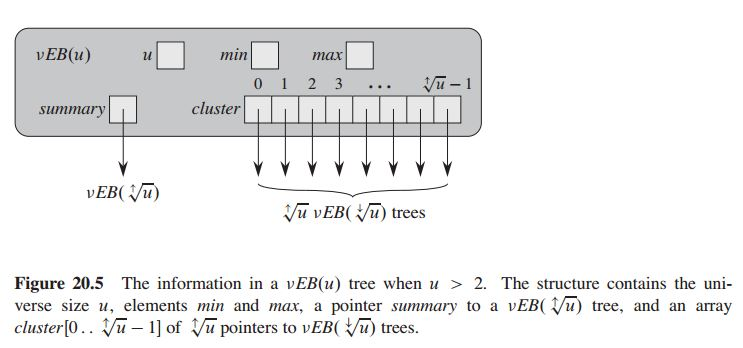
\includegraphics[scale=0.75]{fig/vBE-Struct.JPG}
    \label{fig:vBE-Struct}
    \caption{Estructura vEB - Tomado del Cormen}
\end{figure}

\begin{proposition}[El espacio utilizado por el arbol Van Emde Boas es lineal en la cantidad de elementos del universo de claves]
\end{proposition}
\begin{proof}
Para probar este resultado mostraremos que la recurrencia mencionada en \ref{eq:recurrencia_espacio_vEB} tiene por solucion $\mathcal{O}(u)$. Lo haremos utilizando el teorema maestro.\\
 
 \textbf{Nota: } No estamos teniendo en cuenta las operaciones de techo y piso sobre la raiz cuadrada, pero esto no modifica el comportamiento asintótico de la recurrencia.
 
 Sea la recurrencia modelo del teorema maestro:
 
 \begin{equation}
    \label{eq:recurrencia_teorema_maestro}
    P(u) = aP(\frac{u}{b}) + f(n)
\end{equation}
 
 Identifiquemos en la ecuacion \ref{eq:recurrencia_espacio_vEB} las componentes de la recurrencia generica:
 
\begin{itemize}
    \item Sea $a = (\sqrt{u} + 1)$
    \item Dado que $\sqrt{u} = \frac{u}{\sqrt{u}}$ luego $b = \sqrt{u}$
    \item Por ultimo, $f(u) = \sqrt{u} = u^{0.5}$. Por lo tanto $c = 0.5$
    \item Tenemos $P(u) = (\sqrt{u}+1)P(\frac{u}{\sqrt{u}}) + \mathcal{O}(U^{0.5})$
\end{itemize}
Veamos que aplica el caso 1 del teorema maestro:
\begin{itemize}
\item $f(u) \in \mathcal{O}(u^{\frac{1}{2}})$ y $\frac{1}{2} < 1 < \frac{log_{10}(\sqrt{u}+1)}{log_{10}(\sqrt{u})} = log_{(\sqrt{u} + 1)}(\sqrt{u})$
\item Esta última cota vale porque al ser logaritmo una funcion creciente $\lim_{x \to \infty} \frac{log_{10}(\sqrt{u}+1)}{log_{10}(\sqrt{u})} = 1$ por derecha.
\item En definitiva, al cumplir las hipótesis del caso 1 del teorema maestro: $P(u) \in \mathcal{O}(u)$ como queríamos ver.
\end{itemize}
\end{proof}

\subsection{Item b)}
En la estructura recursiva original vEB de la figura \ref{fig:vBE-Struct}, se tiene:
\begin{itemize}
    \item atributos u, min, max
    \item puntero a summary de tipo vEB($\sqrt{u}$)
    \item $\sqrt{u}$ punteros a estructuras vEB($\sqrt{u}$)
    \item Notar que los hijos nunca son nulos, es decir, aunque ese cluster este vacío igualmente las estructuras hijo existen. \textbf{Esto usa espacio innecesariamente, posiblemente en detrimento de una mayor performance temporal.}. Esto puede verse en la figura \ref{fig:vBE-Ejemplo_Arbol}
\end{itemize}

\begin{figure}[H]
    \centering
    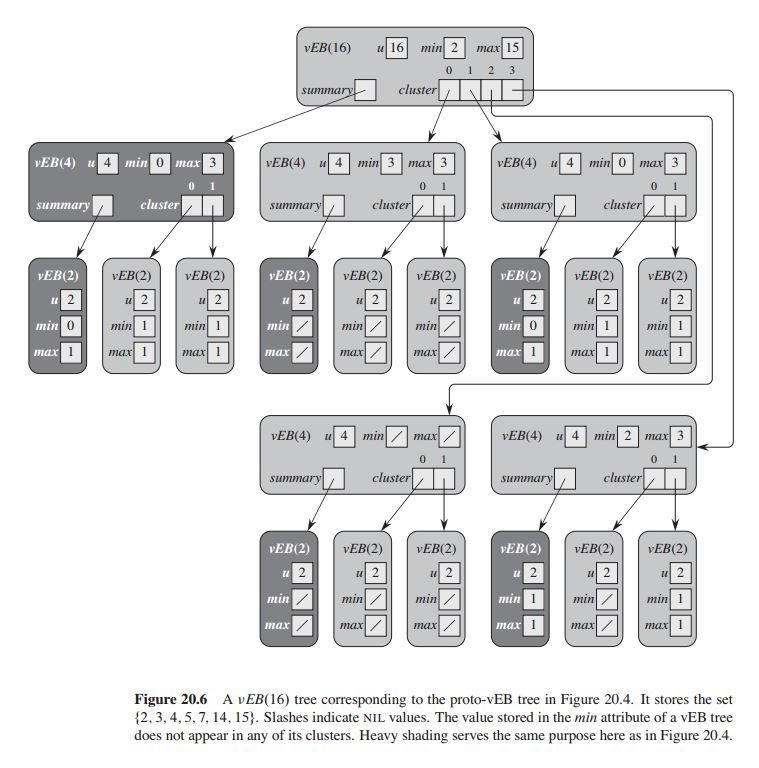
\includegraphics[scale=0.75]{fig/Full-vBE.JPG}
    \label{fig:vBE-Ejemplo_Arbol}
    \caption{Arbol de ejemplo - Tomado del Cormen}
\end{figure}

Hagamos algunas modificaciones:

\begin{itemize}
\item Modifiquemos la semántica de almacenamiento del \texttt{summary}, si este puntero es nulo, indica que todos los clusters están vacíos. Caso contrario, apunta a una estructura vEB de tamaño $\sqrt{u}$ como siempre.
\item Consideremos utilizar una tabla dinámica\footnote{Sección 17.4 del Cormen - Podria por ejemplo, considerarse una tabla de hash con funcion de hashing uniforme} en lugar de un arreglo para almacenar los punteros del cluster de un nodo vEB. 
\item En esta nueva forma de almacenar el cluster de cada nodo, \textbf{solo guardamos los punteros a los clusteres hijos no vacios}, si el elemento i-esimo no se encuentra en la tabla, corresponde a un cluster vacío.
\end{itemize}

Con estas modificaciones logramos que en cada nodo vEB tenga una cantidad de hijos proporcional a la cantidad de clusteres no vacíos.\\

La lógica de las operaciones del árbol se ve alterada por este cambio de estructuras de datos, pero no demasiado, pues se puede proveer una interfaz idéntica a la de un vector en la tabla dinámica, con costos probabilísticos iguales a los de un simple arreglo y mantener así las complejidades temporales de las operaciones. \textbf{Se debe tener en cuenta que hay que agregar validaciones en casos donde el elemento i-esimo de la tabla dinámica sea NIL en las recursiones de las operaciones}. Por otro lado hay que verificar los casos donde haya que crear en tiempo real las estructuras hijas que no se encuentren instanciadas, por ejemplo al insertar un nuevo elemento. O el problema análogo de borrar elementos y dejar el árbol con una estructura interna con summary's instanciados para clusteres vacíos, en este caso se debe liberar la memoria que ya no se necesita. Por último, asumimos que las llamadas a las funciones de reserva o liberación de memoria toman tiempo constante.\\

Con esto en mente y utilizando como base el pseudo-código de las operaciones de la bibliografía\footnote{Páginas 550-555 del Cormen - Tercera edición}, observamos que:
\begin{itemize}
\item El costo de crear un nuevo vEB Tree vacío con las nuevas reglas es de tiempo constante pues no instancia la estructura completa como en la versión original.
\item Las operaciones Mínimo y Máximo quedan sin cambios.
\item La operacion Pertenece, ahora utiliza una tabla dinámica en lugar de un arreglo en la llamada recursiva, deberia haber una condicion de corte si dicho item es nulo, para no iterar sobre una estructura vacía. La complejidad queda probabilísticamente sin cambios.
\item La operacion Sucesor, queda sin cambios, agregando nuevamente validaciones para no hacer recursión en estructuras vacias poniendo condiciones de corte. Nuevamente la complejidad queda probabilísticamente sin cambios respecto al vEB original.
\item La operacion Predecesor, casi análoga a Sucesor, considerando que los mínimos no se guardan en clusters, queda con un análisis similar a la operacion Sucesor, que mantiene su complejidad temporal, pero de forma probabilística por las llamadas a operaciones de la tabla dinámica.

\item Las operaciones de inserción deben subsanar el hecho de que la estructura interna puede estar incompleta. En particular, \textbf{en los casos recursivos} de esta operación donde se inserta el valor correspondiente\footnote{Podria intercambiarse con el mínimo actual si el elemento es mas pequeño que el mínimo.}\texttt{(llamemos x a este valor)} en el árbol, tenemos 2 casos. En lugar de preguntar si el mínimo del cluster apuntado por high(x) es NIL, podemos preguntar si existe dicha entrada en la tabla dinámica para saber cual es el caso que corresponde. 
    \begin{enumerate}
        \item El cluster donde se va a insertar x corresponde a un vEB de tamaño mayor que 2 que está vacío\footnote{Si todos los clústeres estaban vacíos, se crea en tiempo constante \textbf{un solo nivel de recursion hacia abajo del resumen} inicializando todos los punteros a NIL y la tabla vacía. Al hacer recursión para actualizar el resumen, al ser una estructura vacía, se actualiza en una sola llamada recursiva.}: 
        Debemos actualizar el resumen y se llama recursivamente para agregar la información del nuevo cluster al resumen. Por otro lado, inicializar el nuevo cluster\textbf{(un solo nivel de recursión)} toma tiempo constante y asignar mínimo y máximo tambien.
        
        \item El cluster donde se va a insertar x corresponde a un vEB de tamaño mayor que 2 no vacío: En este caso el resumen ya contiene la información acerca de este cluster. Asi que solo resta insertar el elemento recursivamente. En este caso al estar no vacío, esta llamada no cambia respecto del árbol original.
        
    \end{enumerate}
    Notemos que entonces, en la operacion de inserción a lo sumo se crean un resumen y n clusters, al tener tablas dinámicas en lugar de arreglos y no tener mas hijos, es decir, instanciar un solo nivel de recursion hacia abajo, la memoria consumida en cada llamada a inserción es a lo sumo $\mathcal{O}(1)$. Totalizando un espacio máximo consumido por inserción de órden $\mathcal{O}(n)$. De esta forma un árbol vacío consume espacio O(1) y a medida que agregamos elementos, el espacio consumido queda en función de n\footnote{Cantidad de elementos en el arbol} \footnote{Asumiendo limpieza de estructuras innecesarias en borrado}
    
\item La operación de borrado debe tener en cuenta la limpieza de la estructura interna en caso que corresponda. Al borrar un elemento, en caso de quedar un cluster vacío, debe liberarse y eliminarse de la tabla dinámica del padre, posteriormente, hay que actualizar el resumen. Asimismo al estar todos los clústeres vacíos, debe liberarse el resumen y marcarse como nulo el puntero del padre. Estas reglas tambien valen para las estructuras recursivas de los resúmenes.

\end{itemize}

De esta forma no es necesario tener en memoria un espacio reservado del tamaño del universo de claves, teniendo solo en memoria las estructuras necesarias para la cantidad de elementos actualmente en el conjunto. El costo que se paga en complejidad temporal por esta mejora es que algunas operaciones ahora quedan con complejidades probabilísticas, ya que usan una tabla dinámica, por ejemplo una funcion de hash con funcion de hasheo uniforme.

\end{document}
